\documentclass[letterpaper,12pt]{article}\usepackage[]{graphicx}\usepackage[]{color}
%% maxwidth is the original width if it is less than linewidth
%% otherwise use linewidth (to make sure the graphics do not exceed the margin)
\makeatletter
\def\maxwidth{ %
  \ifdim\Gin@nat@width>\linewidth
    \linewidth
  \else
    \Gin@nat@width
  \fi
}
\makeatother

\definecolor{fgcolor}{rgb}{0.345, 0.345, 0.345}
\newcommand{\hlnum}[1]{\textcolor[rgb]{0.686,0.059,0.569}{#1}}%
\newcommand{\hlstr}[1]{\textcolor[rgb]{0.192,0.494,0.8}{#1}}%
\newcommand{\hlcom}[1]{\textcolor[rgb]{0.678,0.584,0.686}{\textit{#1}}}%
\newcommand{\hlopt}[1]{\textcolor[rgb]{0,0,0}{#1}}%
\newcommand{\hlstd}[1]{\textcolor[rgb]{0.345,0.345,0.345}{#1}}%
\newcommand{\hlkwa}[1]{\textcolor[rgb]{0.161,0.373,0.58}{\textbf{#1}}}%
\newcommand{\hlkwb}[1]{\textcolor[rgb]{0.69,0.353,0.396}{#1}}%
\newcommand{\hlkwc}[1]{\textcolor[rgb]{0.333,0.667,0.333}{#1}}%
\newcommand{\hlkwd}[1]{\textcolor[rgb]{0.737,0.353,0.396}{\textbf{#1}}}%
\let\hlipl\hlkwb

\usepackage{framed}
\makeatletter
\newenvironment{kframe}{%
 \def\at@end@of@kframe{}%
 \ifinner\ifhmode%
  \def\at@end@of@kframe{\end{minipage}}%
  \begin{minipage}{\columnwidth}%
 \fi\fi%
 \def\FrameCommand##1{\hskip\@totalleftmargin \hskip-\fboxsep
 \colorbox{shadecolor}{##1}\hskip-\fboxsep
     % There is no \\@totalrightmargin, so:
     \hskip-\linewidth \hskip-\@totalleftmargin \hskip\columnwidth}%
 \MakeFramed {\advance\hsize-\width
   \@totalleftmargin\z@ \linewidth\hsize
   \@setminipage}}%
 {\par\unskip\endMakeFramed%
 \at@end@of@kframe}
\makeatother

\definecolor{shadecolor}{rgb}{.97, .97, .97}
\definecolor{messagecolor}{rgb}{0, 0, 0}
\definecolor{warningcolor}{rgb}{1, 0, 1}
\definecolor{errorcolor}{rgb}{1, 0, 0}
\newenvironment{knitrout}{}{} % an empty environment to be redefined in TeX

\usepackage{alltt}
\usepackage[top=1in,bottom=1in,left=1in,right=1in]{geometry}
\usepackage{setspace}
\usepackage[colorlinks=true,urlcolor=blue,citecolor=blue,linkcolor=blue]{hyperref}
\usepackage{indentfirst}
\usepackage{multirow}
\usepackage{booktabs}
\usepackage[final]{animate}
\usepackage{graphicx}
\usepackage{verbatim}
\usepackage{rotating}
\usepackage{tabularx}
\usepackage{array}
\usepackage{subfig} 
\usepackage[noae]{Sweave}
\usepackage{cleveref}
\usepackage[figureposition=bottom]{caption}
\usepackage{paralist}
\usepackage{acronym}
\usepackage{outlines}
\usepackage{pdflscape}

% housekeeping


\linespread{1}
\IfFileExists{upquote.sty}{\usepackage{upquote}}{}
\begin{document}
\title{Analysis of crab abundance, presence/absence, and carapace length}
\maketitle



\begin{knitrout}
\definecolor{shadecolor}{rgb}{0.969, 0.969, 0.969}\color{fgcolor}
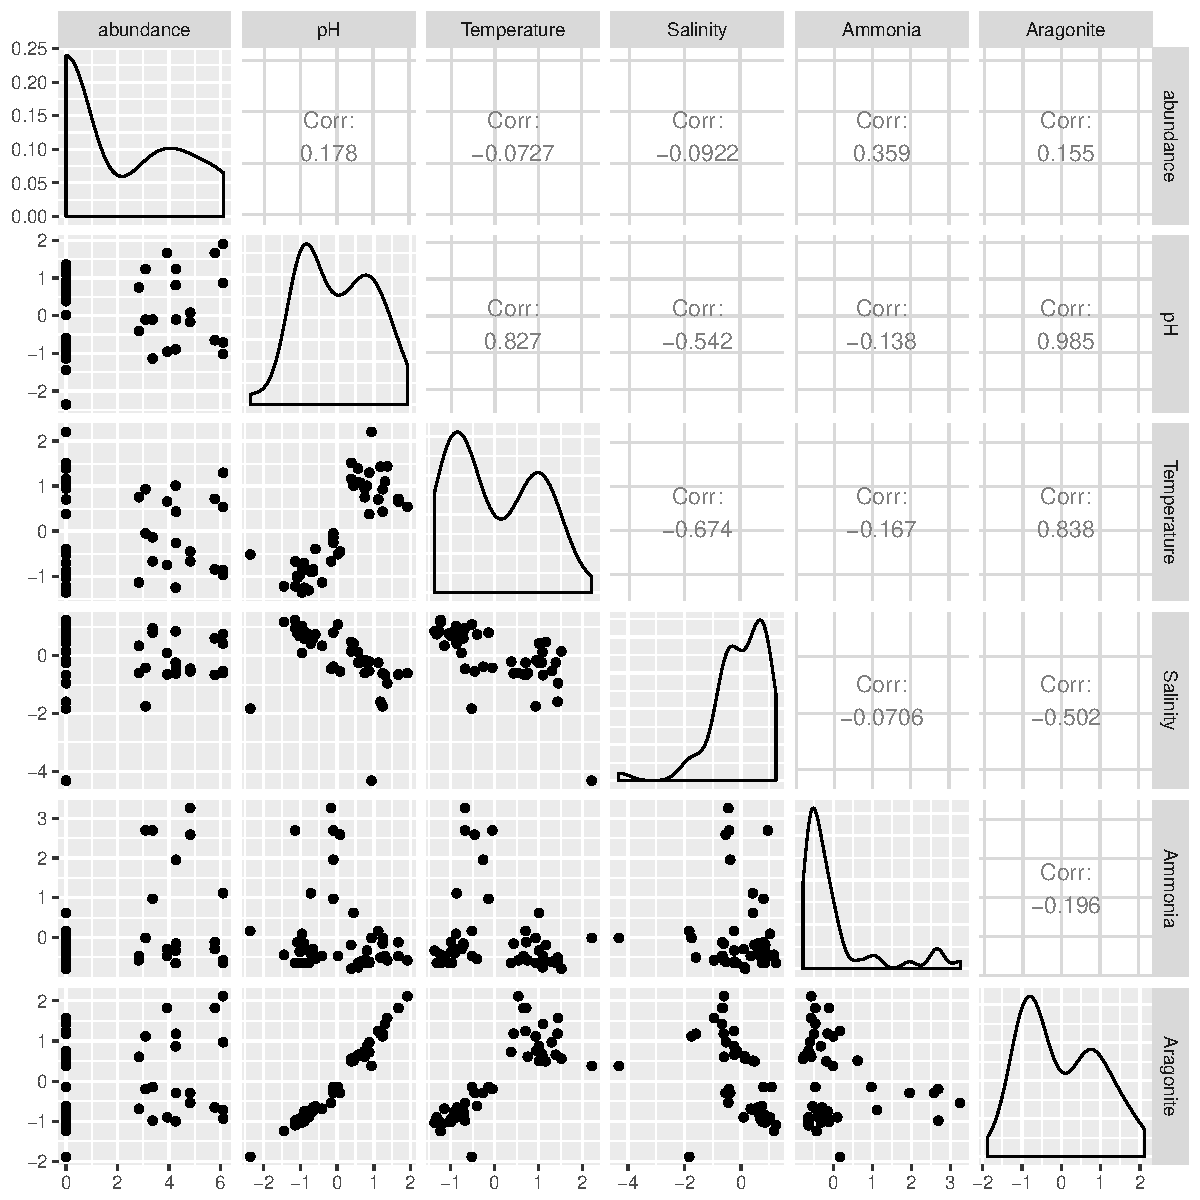
\includegraphics[width=\maxwidth]{figure/unnamed-chunk-3-1} 

\end{knitrout}



\begin{knitrout}
\definecolor{shadecolor}{rgb}{0.969, 0.969, 0.969}\color{fgcolor}\begin{figure}
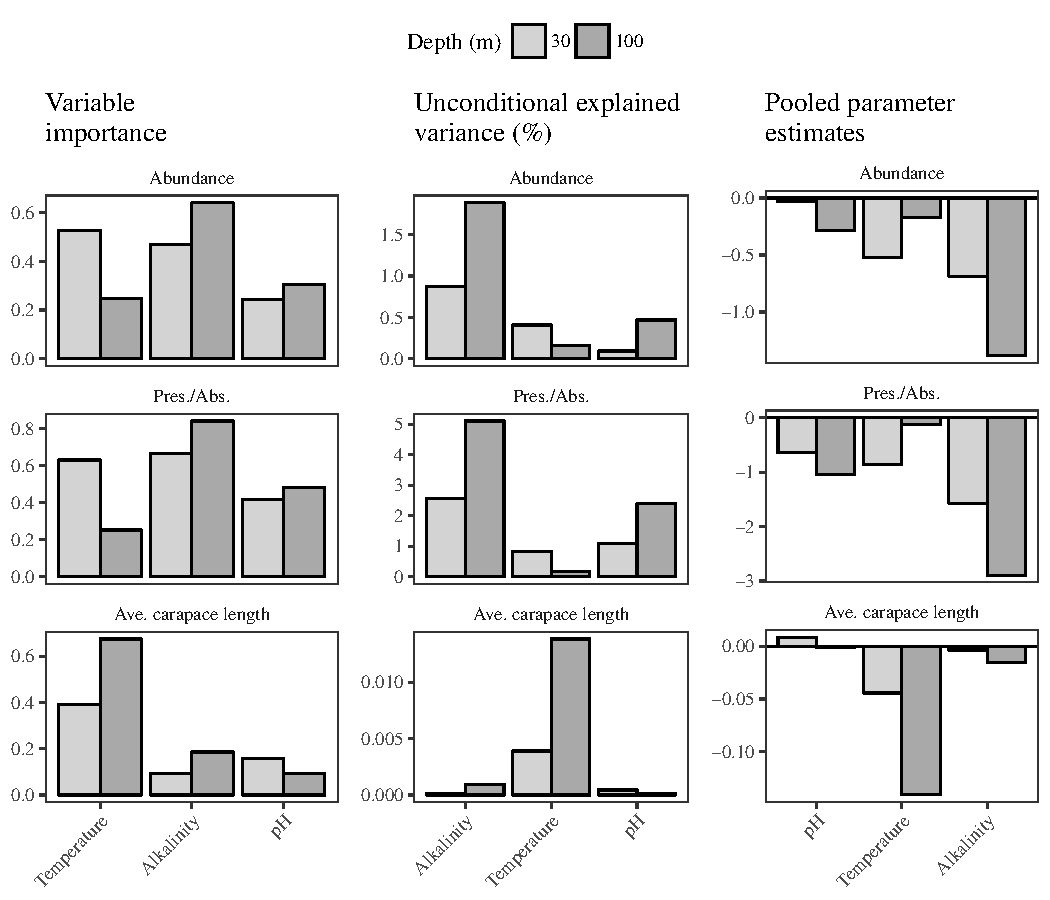
\includegraphics[width=\maxwidth]{figure/unnamed-chunk-5-1} \caption[Results of model selection analysis with three crab population variables (abundance, presence/absence, carapace length) by shallow and deep water]{Results of model selection analysis with three crab population variables (abundance, presence/absence, carapace length) by shallow and deep water. Variable importances and pooled estimates show summarized results from multiple models that evaluated all parameter combinations.  The unconditional explained variance (\%) is the effect of each variable independent of all other variables.}\label{fig:unnamed-chunk-5}
\end{figure}


\end{knitrout}
\clearpage

\begin{landscape}
\centering\vspace*{\fill}
%latex.default(abutab[, -c(1, 2)], file = "", rowlabel = "Models",     caption = cap.val, caption.loc = "top", rgroup = names(table(abutab$depth)),     n.rgroup = table(abutab$depth), rowname = abutab$model, size = "scriptsize",     label = "tab:abutab")%
\begin{table}[!tbp]
{\scriptsize
\caption{Top five selected models for crab abundance at shallow and deep water. Input variables were aragonite, oxygen, ph, salinity, and temperature. All explanatory variables were scaled and centered.\label{tab:abutab}} 
\begin{center}
\begin{tabular}{lllllllllll}
\hline\hline
\multicolumn{1}{l}{Models}&\multicolumn{1}{c}{Int.}&\multicolumn{1}{c}{Aragonite}&\multicolumn{1}{c}{Oxygen}&\multicolumn{1}{c}{pH}&\multicolumn{1}{c}{Salinity}&\multicolumn{1}{c}{Temperature}&\multicolumn{1}{c}{df}&\multicolumn{1}{c}{logLik}&\multicolumn{1}{c}{AICc}&\multicolumn{1}{c}{delta}\tabularnewline
\hline
{\bfseries 100 m}&&&&&&&&&&\tabularnewline
~~1&2.34&-&-&-&-1.76&-1.01&4&-48.29&106.8&0\tabularnewline
~~2&1.75&-&-&-&-1.51&-&3&-50.42&108.11&1.31\tabularnewline
~~3&2.54&-&-&-1.3&-2.39&-&4&-49.01&108.24&1.44\tabularnewline
~~4&2.44&-1.02&-&-&-2.09&-&4&-49.28&108.77&1.97\tabularnewline
~~5&1.94&-&-&-&-&-&2&-52.17&108.94&2.14\tabularnewline
\hline
{\bfseries 30 m}&&&&&&&&&&\tabularnewline
~~1&2.75&-&-&-&-1.85&-&3&-49.78&106.83&0\tabularnewline
~~2&2.52&-&-&-1.25&-2.81&-&4&-48.86&107.94&1.11\tabularnewline
~~3&2.26&-&-&-&-2.21&-0.99&4&-48.98&108.17&1.34\tabularnewline
~~4&2.31&-1.28&-&-&-2.53&-&4&-49.02&108.26&1.43\tabularnewline
~~5&2.59&-&-0.81&-&-2.65&-&4&-49.31&108.84&2.01\tabularnewline
\hline
\end{tabular}\end{center}}
\end{table}
%latex.default(patab[, -c(1, 2)], file = "", rowlabel = "Models",     caption = cap.val, caption.loc = "top", rgroup = names(table(patab$depth)),     n.rgroup = table(patab$depth), rowname = patab$model, size = "scriptsize",     label = "tab:patab")%
\begin{table}[!tbp]
{\scriptsize
\caption{Top five selected models for crab presence/absence at shallow and deep water. Input variables were aragonite, oxygen, ph, salinity, and temperature. All explanatory variables were scaled and centered.\label{tab:patab}} 
\begin{center}
\begin{tabular}{lllllllllll}
\hline\hline
\multicolumn{1}{l}{Models}&\multicolumn{1}{c}{Int.}&\multicolumn{1}{c}{Aragonite}&\multicolumn{1}{c}{Oxygen}&\multicolumn{1}{c}{pH}&\multicolumn{1}{c}{Salinity}&\multicolumn{1}{c}{Temperature}&\multicolumn{1}{c}{df}&\multicolumn{1}{c}{logLik}&\multicolumn{1}{c}{AICc}&\multicolumn{1}{c}{delta}\tabularnewline
\hline
{\bfseries 30}&&&&&&&&&&\tabularnewline
~~1&1.08&-&-&-2.79&-4.17&-&3&-10.51&28.28&0\tabularnewline
~~2&0.28&-&-&-&-2.25&-1.79&3&-10.97&29.2&0.92\tabularnewline
~~3&1&-2.27&-&-&-3.29&-&3&-11.07&29.39&1.11\tabularnewline
~~4&1.06&-&-&-1.92&-3.81&-0.97&4&-9.98&30.18&1.9\tabularnewline
~~5&0.76&-&-1.13&-&-3.46&-1.6&4&-10.24&30.7&2.42\tabularnewline
\hline
{\bfseries 100}&&&&&&&&&&\tabularnewline
~~1&0.87&-&-&-2.2&-4.94&-&3&-10.61&28.48&0\tabularnewline
~~2&0.84&-&-&-&-2.62&-&2&-12.21&29.01&0.54\tabularnewline
~~3&0.36&-2.21&-&-&-4.19&-&3&-10.91&29.08&0.6\tabularnewline
~~4&0.86&-&-1.48&-&-4.54&-&3&-11.15&29.57&1.09\tabularnewline
~~5&0.77&-&6.04&-9.31&-4.35&-&4&-9.85&29.92&1.45\tabularnewline
\hline
\end{tabular}\end{center}}
\end{table}

\end{landscape}

\begin{landscape}
\centering\vspace*{\fill}
%latex.default(cltab[, -c(1, 2)], file = "", rowlabel = "Models",     caption = cap.val, caption.loc = "top", rgroup = names(table(cltab$depth)),     n.rgroup = table(cltab$depth), rowname = cltab$model, size = "scriptsize",     label = "tab:cltab")%
\begin{table}[!tbp]
{\scriptsize
\caption{Top five selected models for crab carapace length at shallow and deep water. Input variables were aragonite, oxygen, ph, salinity, and temperature.  All explanatory variables were scaled and centered.\label{tab:cltab}} 
\begin{center}
\begin{tabular}{lllllllllll}
\hline\hline
\multicolumn{1}{l}{Models}&\multicolumn{1}{c}{Int.}&\multicolumn{1}{c}{Aragonite}&\multicolumn{1}{c}{Oxygen}&\multicolumn{1}{c}{pH}&\multicolumn{1}{c}{Salinity}&\multicolumn{1}{c}{Temperature}&\multicolumn{1}{c}{df}&\multicolumn{1}{c}{logLik}&\multicolumn{1}{c}{AICc}&\multicolumn{1}{c}{delta}\tabularnewline
\hline
{\bfseries 30}&&&&&&&&&&\tabularnewline
~~1&6.59&-&-&-&-&-&2&6.99&-8.28&0\tabularnewline
~~2&6.6&-&-&-&-&-0.09&3&8.57&-7.14&1.13\tabularnewline
~~3&6.57&-&-&0.11&-&-0.2&4&10.45&-4.9&3.38\tabularnewline
~~4&6.6&-0.03&-&-&-&-&3&7.34&-4.68&3.6\tabularnewline
~~5&6.6&-&-&-0.02&-&-&3&7.12&-4.23&4.04\tabularnewline
\hline
{\bfseries 100}&&&&&&&&&&\tabularnewline
~~1&6.45&-&-&-&-&-0.19&3&9.82&-9.64&0\tabularnewline
~~2&6.59&-&-&-&-&-&2&6.99&-8.28&1.37\tabularnewline
~~3&6.42&-0.63&-&0.41&-&-&4&12.07&-8.14&1.5\tabularnewline
~~4&6.41&-&-&-&-0.1&-0.27&4&11.68&-7.35&2.29\tabularnewline
~~5&6.46&-0.42&0.23&-&-&-&4&11.25&-6.5&3.15\tabularnewline
\hline
\end{tabular}\end{center}}
\end{table}

\end{landscape}

\end{document}
